\documentclass[letterpaper]{article}
\usepackage{geometry}
\usepackage{xcolor}
\usepackage{amsmath}
\usepackage[some]{background}
\usepackage{lipsum}

\definecolor{titlepagecolor}{cmyk}{1,.60,0,.40}
\definecolor{titlepagecolor2}{rgb}{19, 62, 135}

\DeclareFixedFont{\bigsf}{T1}{phv}{b}{n}{1.5cm}

\backgroundsetup{scale=1,angle=0,opacity=1,contents={\begin{tikzpicture}[remember picture,overlay]
 \path [fill=titlepagecolor] (-0.5\paperwidth,5) rectangle (0.5\paperwidth,10);  
\end{tikzpicture}}
}
\makeatletter
\def\printauthor{%                  
    {\large \@author}}              
\makeatother
\author{%
    Gagik Gavalian \\
    Harut Avakian \\
    Patrick Achenbach \\
    Richard Tyson \\
    \textit{Jefferson Lab, Newport News, VA, USA }\vspace{40pt} \\
     Aleksandr Privalov \\
    \textit{NIIChaVo}
    }
\begin{document}
\begin{titlepage}
\BgThispage
\newgeometry{left=1cm,right=4cm}
\vspace*{4cm}
\noindent
\textcolor{white}{
%\bigsf
\huge 
\textsf{Integration of AI/ML in experimental data  lifecycle in CLAS12}}
\vspace*{2.5cm}\par
\noindent
\begin{minipage}{0.35\linewidth}
    \begin{flushright}
        \printauthor
    \end{flushright}
\end{minipage} \hspace{15pt}
%
\begin{minipage}{0.02\linewidth}
    \rule{1pt}{175pt}
\end{minipage} \hspace{-10pt}
%
\begin{minipage}{0.8\linewidth}
\vspace{5pt}
    \begin{abstract} 
 Artificial Intelligence and Machine Learning (AI/ML) algorithms have seen a variety of implemented 
    and proof-of-concept applications at the CEBAF Large Acceptance Spectrometer at 12 GeV (CLAS12) located 
    at the Continuous Electron Beam Accelerator Facility (CEBAF). Past applications have focused on data-taking, 
    reconstruction, simulation, and data analysis, whilst several other stages in the process chain will benefit 
    from the full application of AI/ML. This paper introduces a proposal to combine the existing 
    wealth of experience and applications at CLAS12 and implement novel AI/ML-based solutions where they are missing. 
    This implementation aims to improve the overall experimental life cycle, minimizing the time required to produce and 
    publish higher-quality data compared to existing paradigms. This will transform a human-driven nuclear 
    physics experiment into a fully AI/ML-assisted one
    \end{abstract}
\end{minipage}
\end{titlepage}
\restoregeometry

%\lipsum[1-2]



\section{Introduction}


\section{Data Acquisition}


\section{Detector Monitoring}


\section{Reconstruction}


\section{Physics Analysis}

The superior luminosity of CEBAF, high resolutions of detectors, and the ability for multidimensional and multiparticle detection make the Jefferson Lab unique in disentangling the genuine intrinsic transverse structure of hadrons encoded in 3D partonic distributions, including Transverse Momentum Distributions (TMDs)  and Generalized Parton Distributions (GPDs) in the kinematics dominated by valence quarks. Recent studies of exclusive vector mesons performed at JLab indicate understanding of the impact of exclusive vector mesons is important for understanding of underlying GPDs, and absolutely critical for interpretation of Semi-Inclusive Deep Inelastic Scattering processes providing access to TMDs.
Detailed studies of exclusive vector mesons and neutral rho production, in particular, rely on measurements of Spin Density Matrix Elements (SDMEs) describing the spin transfer from the virtual photon to the vector meson.
Studies of TMDs, GPDs, and SDMEs, require measurements of polarization-independent, and spin-dependent azimuthal asymmetries, which are multidifferential in nature. Therefore, a multidimensional analysis is mandatory to unravel the intricate dependencies of the kinematical variables. An example of different angular modulations of the cross-section of exclusive rho, with definitions of angles, is shown in APPENDIX A. Listed are only 15 SDMEs from 23 contributions just for the unpolarized target case. Many more modulations appear with polarized targets. Given that most of the golden measurements planned at the future Electron-Ion Collider include measurements with polarized targets, understanding of the rho contributions will be important both for the interpretation of existing leptoproduction data and also future measurements. 
Separation of different dynamical contributions is very challenging for the QCD based phenomenology, requiring fits in the multidimensional space, and relying on various parameterizations, introducing systematics which is hard to quantify.

We propose a framework for extraction of underlying SDMES, TMDs and GPDs from CLAS12 data sets with polarized beam and unpolarized hydrogen and deuteron, and longitudinally polarized NH3 targets, based on the AI tools for extraction of objects of interest from different stages of physics data analysis, starting from the raw detector response and ending with final event samples, identified and corrected for detector acceptances and efficiencies. 

Extracted physics observables are corrected for detector acceptance and then fitted (usually in one dimension) with a theoretical model to extract parameters. With advancements in AI, the methods of extracting physics model parameters from experimental data haven't significantly changed.
The field of nuclear physics must include more advanced methods in physics analysis. 
We propose to investigate a different approach to extracting theoretical model parameters from experimental data. 
The program must generate events for particular physics reactions based on matrix elements provided by the theoretical model. Several simulations must be made with varying starting parameters of the model (within physical range). The resulting event sample must then be processed with a detector simulation program (using AI, discussion below) to obtain event samples that will be experimentally detectable. Then, a neural network would be trained on multi-dimensional data to learn distributions of each starting theoretical model parameter in real experimental data space. Once the network is trained with sufficient starting input parameters, it can output theoretical model parameters based on experimental distributions.
The method described above relies on obtaining experimental event samples from original theoretical simulated event samples. This process is the most time-consuming in the current data analysis workflow. It requires passing particles through physics simulation programs (usually GEANT), simulating the responses of each detector on the particle path. Then, the reconstruction program must process the detector data and reconstruct the particles, which can be used in physics analysis. This process is computationally intensive and can not be used to process large amounts of data originating from different theoretical models with varying parameters in a reasonable amount of time. To be able to train the physics AI model on large amounts of data, a fast detector emulation program will be needed. 
A fast AI-based detector emulation will be developed, which will process and input physics events emulating detector acceptance and resolutions to produce experimental distributions measured by the detector.
This project will develop infrastructure (software framework) to simulate experimental detectors using Neural Networks, which will be general enough to be used with other detector systems. The network will be trained on the data produced by a more extensive (GEANT-based) detector simulation program to learn the detector acceptance and resolutions. This Neural Network will then be used to produce multi-dimensional physics observables from events generated with given theoretical models. The physics observables generated in such a way will then be used to train another neural network for estimating theoretical model parameters from raw distributions. The experimentally measured distributions can then be evaluated by the later neural networks to extract (predict) the most probable parameters of the theoretical model.

This approach to physics analysis can improve the collaboration between theory and experimental groups as well as between different experiments measuring the same physics observables. Sharing data between experiments is very tedious at present due to the specifics of the detector's knowledge required to analyze the data. With our approach, each experiment can train a Neural Network that will replicate the effect of events being detected in the detector. Theory groups can develop different models for given physics observables with different parameter sets with the ability to produce events. The experimental groups then can train physics neural networks using detector simulation neural networks using theoretical models and then use experimental physics observable distributions to infer parameter sets for specific theoretical models.

In our work, we will apply this approach to one specific physics reaction (i.e. productions of rho meson) and demonstrate the method and future extensibility.


\section{Large Language Models}



\section{Collaboration Projects}

Artificial intelligence and machine learning (AI/ML) are utilized across various components of the CLAS12 experiment, including online data monitoring, offline reconstruction, data analysis, and enhanced particle identification. Their integration into the reconstruction process has led to a substantial improvement in the experiments' statistical precision.

\subsection{AI/ML in CLAS12 tracking}

CLAS12 tracking algorithms employ AI techniques to enhance track reconstruction. A sequence of neural networks operates in concert to maximize efficiency. Initially, a Convolutional Autoencoder is applied to denoise raw signals from the Drift Chambers (DC). Subsequently, a Multi-Layer Perceptron (MLP) connects clusters across the six DC superlayers to identify track candidates. To address inefficiencies such as missing segments in one or more superlayers, a secondary autoencoder is used to recover incomplete tracks. The incorporation of AI into CLAS12 reconstruction has led to a significant increase in tracking efficiency (approximately $20\%$ at a 50 nA electron beam on a hydrogen target), resulting in an estimated $60\%$ gain in collected statistics for three-particle final state reactions.

\begin{figure}[h!]
\centering
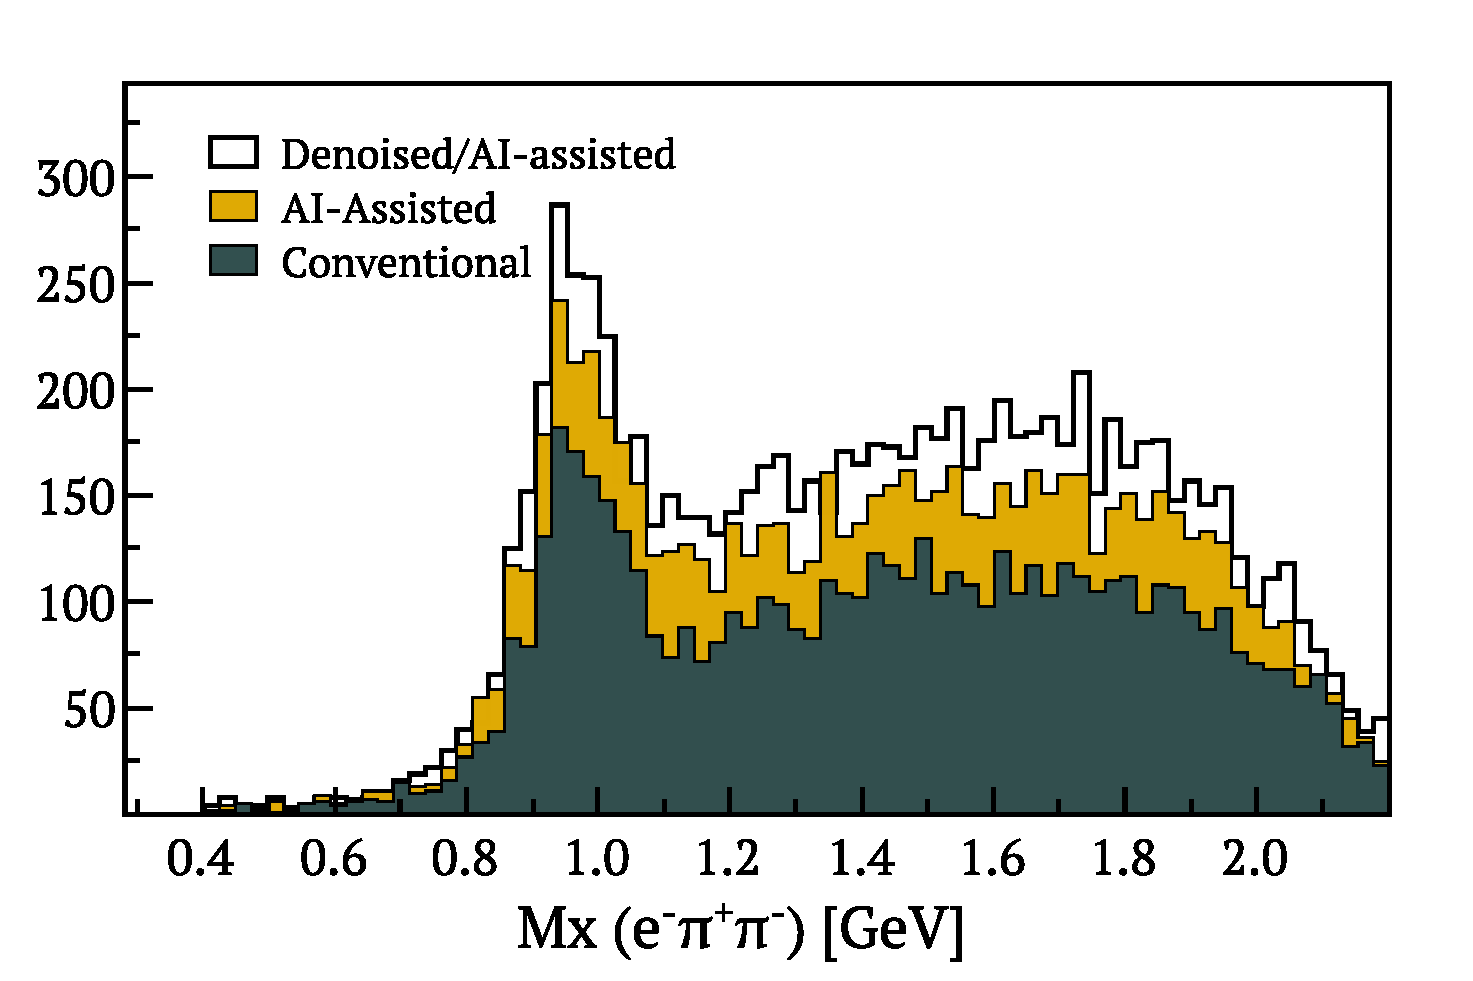
\includegraphics[width=0.42\columnwidth]{images/projects/figure_denoise_mxp.pdf}
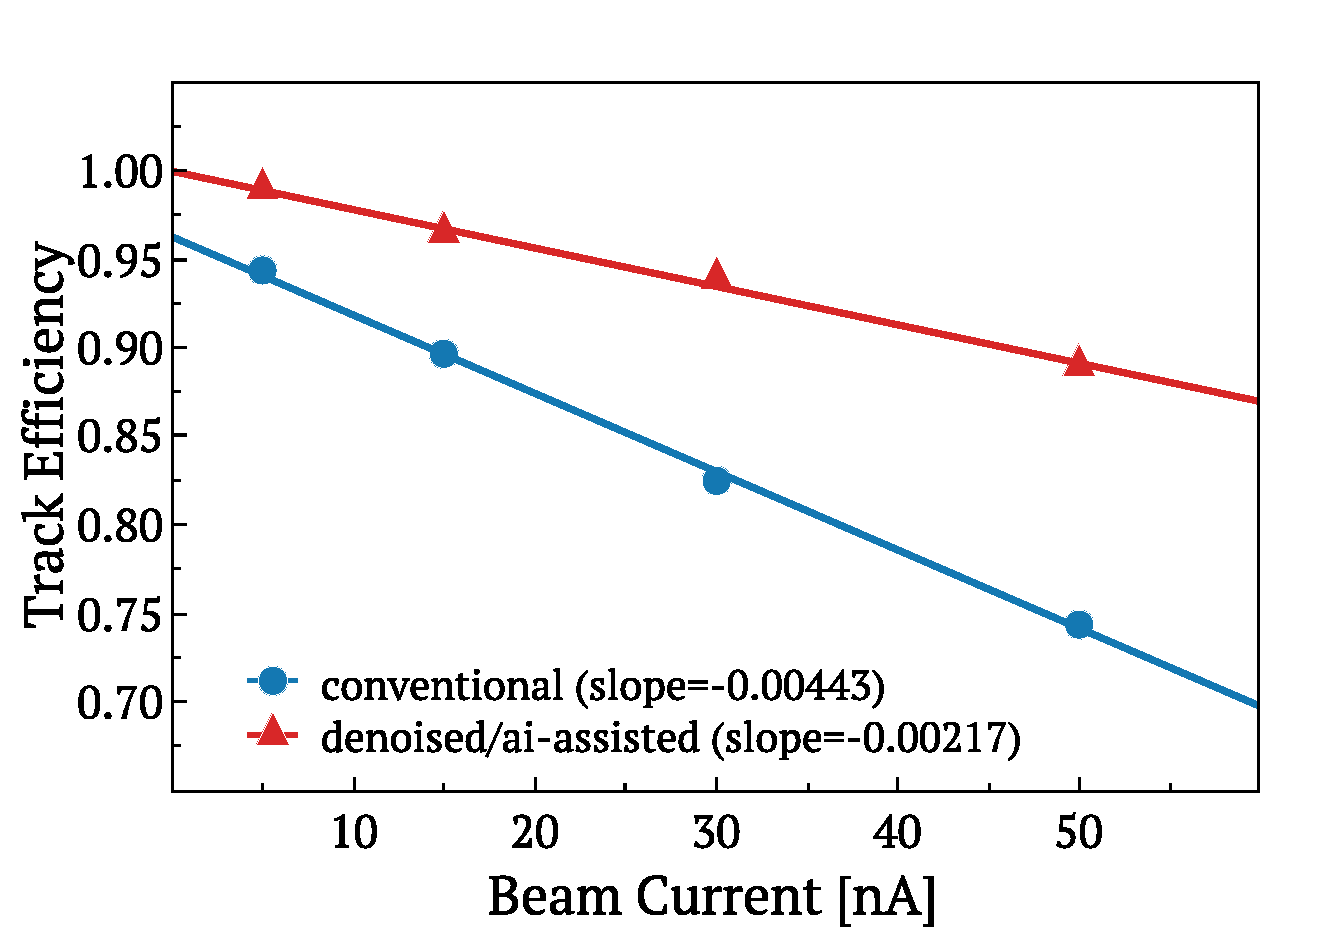
\includegraphics[width=0.42\columnwidth]{images/projects/luminosity_scan.pdf}
\caption{ } 
\label{fig:ai_results}
\end{figure}

Figure~\ref{fig:ai_results} (left) presents the statistical gain for the reaction $H(e) \rightarrow e^\prime\pi^+\pi^-X$, where the missing mass distribution of the detected particles highlights the missing proton. Figure~\ref{fig:ai_results} (right) shows the track reconstruction efficiency as a function of luminosity (beam current), comparing conventional tracking with AI-augmented tracking. The enhanced efficiency achieved through AI integration enables experiments to operate at higher luminosities while maintaining robust track finding performance. AI-augmented track finding has been integrated into the standard data processing workflow and is currently employed in the processing of experimental data.

\subsection{Online Reconstruction in CLAS12}


%\input{data_analysis_data}
%\input{results}

\section{Discussion}



\begin{thebibliography}{00}
\bibitem{AITracking}
P. Thomadakis, A. Angelopoulos, G. Gavalian, \emph{et. al.}, \emph{Comput. Phys. Commun.} \textbf{276} 108360 (2022).

\bibitem{AITracking2}
G. Gavalian, \emph{et. al.}, R. De Vita, V. Ziegler, \emph{ArXiv e-prints} arXiv:2202.06869 (2022).

\bibitem{AIDenoising}
P. Thomadakis, A. Angelopoulos, G. Gavalian, \emph{et. al.}, \emph{Comput. Phys. Commun.} \textbf{271} 108201 (2022).

\bibitem{FastSim}
D. Darulis, R. Tyson, \emph{et. al.}, \emph{ArXiv e-prints} arXiv:2207.11254 (2022).

\bibitem{InstaRec}
G. Gavalian, \emph{JINST} \textbf{19} C05050 (2024).

\bibitem{Hydra}
T. Jeske, \emph{et. al.}, \emph{EPJ Web of Conf.} \textbf{295} 02008 (2024).

\end{thebibliography}

\end{document}
